\documentclass{exercise}

\institute{Institut für Statistik und Wirtschaftsmathematik}
\title{Präsenzübung 1}
\author{Joshua Feld, 406718}
\course{Statistik}
\professor{Cramer}
\semester{Sommersemester 2022}
\program{CES (Bachelor)}

\begin{document}
    \maketitle


    \section*{Aufgabe 1}

    \begin{problem}
        Ordnen Sie den folgenden Merkmalen jeweils einen der Merkmalstypen
        \begin{quote}
            qualitativ/nominal, qualitativ/ordinal, quantitativ/diskret, quantitativ/stetig.
        \end{quote}
        zu, und geben Sie zu jedem Merkmal mögliche Ausprägungen an.
        Geben Sie weiter an, welches der Merkmale verhältnisskaliert ist.
        \begin{itemize}
            \item Alter
            \item Familienstand
            \item Geschlecht
            \item Einkommen (pro Jahr)
            \item Schulbildung
            \item Beruf
            \item Schulnote
            \item Körpergewicht
            \item Intelligenzquotient
            \item Temperatur
        \end{itemize}
    \end{problem}
    
    \subsection*{Lösung}
    \begin{center}
        \begin{tabular}{lcc}
            \toprule
            Merkmal & Merkmalstyp & Mögiche Ausprägungen\\
            \midrule
            Alter & \makecell{quantitativ/diskret\\(verhältnisskaliert)} & \(1, 2, 3, \ldots\)\\
            Familienstand & qualitativ/nominal & ledig, verheiratet, geschieden\\
            Geschlecht & \makecell{qualitativ/nominal\\(dichotom)} & \makecell{männlich, weiblich\\\(1\), \(0\) (bei entsprechender Codierung)}\\
            Einkommen (pro Jahr) & \makecell{quantitativ/diskret\\(verhältnisskaliert)} & \(4920\text{\euro}\), \(48475,35\text{\euro}, \ldots\)\\
            Schulbildung & qualitativ/ordinal & Realschulabschluss, Fachabitur, Abitur\\
            Beruf & qualitativ/nominal & Bäcker, Maler, Mathematikerin, etc.\\
            Schulnote & qualitativ/ordinal & sehr gut, gut, etc.\\
            Körpergewicht & \makecell{quantitativ/stetig\\(verhältnisskaliert)} & \(14,2457\sis{\kilo\gram}, 45,4224\sis{\kilo\gram}, \ldots\)\\
            Intelligenzquotient & \makecell{quantitativ/diskret\\(verhältnisskaliert)} & \(65, 156, \ldots\)\\
            Temperatur & quantitativ/stetig & \(1\sis{\kelvin}, 10\si{\degreeCelsius}, 23\si{\degreeFahrenheit}, \ldots\)\\
            \bottomrule
        \end{tabular}
    \end{center}


    \section*{Aufgabe 2}

    \begin{problem}
        Eine Firma produziert elektronische Bauteile, die im Anschluss an die Herstellung einer Qualitätskontrolle unterzogen werden.
        Im Rahmen dieser Überprüfung wurden im Zeitraum eines Jahres für die einzelnen Quartale die folgenden Anzahlen aussortierter Bauteile ermittelt:
        \begin{center}
            \begin{tabular}{lcccc}
                \toprule
                Quartal & \(1\) & \(2\) & \(3\) & \(4\)\\
                \midrule
                Anzahl aussortierter Bauteile & \(3000\) & \(2800\) & \(2400\) & \(2000\)\\
                \bottomrule
            \end{tabular}
        \end{center}
        Erstellen Sie ein Kreisdiagramm zu den gegebenen Quartalszahlen der aussortierten Bauteile.
    \end{problem}

    \subsection*{Lösung}
    Den Winkel \(\varphi_i\) im Kreisdiagramm für die Anzahl der aussortierten Bauteile in Quartal \(i\) für \(i \in \braces*{1, \ldots, 4}\) berechnet man gemäß der Formel
    \[
        \varphi_i = f_i \cdot 360^\circ.
    \]
    Hierbei bezeichnet \(f_i\) die relative Häufigkeit in Quartal \(i \in \braces*{1, \ldots, 4}\), welche in der folgenden Tabelle auf drei Nachkommastellen gerundet wird.
    \begin{center}
        \begin{tabular}{cccc}
            \toprule
            Quartal & Anzahl aussortierter Bauteile & rel. Häufigkeiten & Winkel in Grad im Kreisdiagramm\\
            \midrule
            \(1\) & \(3000\) & \(0,294\) & \(105,84\)\\
            \(2\) & \(2800\) & \(0,275\) & \(99\)\\
            \(3\) & \(2400\) & \(0,235\) & \(84,6\)\\
            \(4\) & \(2000\) & \(0,196\) & \(70,56\)\\
            \midrule
            Summe & \(10200\) & \(1\) & \(360\)\\
            \bottomrule
        \end{tabular}
    \end{center}
    \begin{center}
        \begin{tikzpicture}
            \pie[radius=2,color={white,white,white,white}] {29.4/1. Quartal,27.5/2. Quartal,23.5/3. Quartal,19.6/4. Quartal};
        \end{tikzpicture}
    \end{center}


    \section*{Aufgabe 3}

    \begin{problem}
        Ein Fahrzeughersteller hat die Zufriedenheit seiner Kunden mit einem bestimmten Fahrzeugtyp untersucht.
        Hierzu wurden zwanzig Kunden gebeten, die Qualität ihres Fahrzeugs einzustufen.
        Es wurden folgende Bewertungen vorgenommen:
        \begin{quote}
            \emph{schlecht, hervorragend, gut, mittelmäßig, gut, hervorragend, gut, sehr schlecht, sehr schlecht, schlecht, gut, mittelmäßig, gut, schlecht, sehr schlecht, schlecht, sehr schlecht, gut, mittelmäßig, gut.}
        \end{quote}
        \begin{enumerate}
            \item
            \begin{enumerate}
                \item Ordnen Sie dem Merkmal \emph{Fahrzeugqualität} einen geeigneten Merkmalstypen zu.
                \item Berechnen Sie zu den verschiedenen aufgetretenen Merkmalsausprägungen die zugehörigen absoluten und relativen Häufigkeiten.
                Stellen Sie weiter die relativen Häufigkeiten mittels eines Säulendiagramms dar.
                \item Bestimmen Sie zu den Fahrzeugbewertungen die zugehörigen Modalwerte (d.h. die Ausprägungen mit maximaler Häufigkeit unter den verschiedenen Fahrzeugbewertungen).
            \end{enumerate}
            \item Beschreiben Sie die Merkmalsausprägungen \emph{hervorragend, \(\ldots\), sehr schlecht} durch die Notenskala \(1, \ldots, 5\) (in dieser Reihenfolge).
            Bestimmen Sie zu den auf diese Weise kodierten zwanzig angegebenen Fahrzeugbewertungen die zugehörige Rangwertreihe sowie die Ränge der einzelnen Fahrzeugbewertungen.
        \end{enumerate}
    \end{problem}

    \subsection*{Lösung}
    \begin{enumerate}
        \item
        \begin{enumerate}
            \item Merkmalstyp: qualitativ/ordinal, darstellbar z.B. durch die Ziffern \(1, \ldots, 5\) (Noten).
            \item Es ergibt sich folgende Tabelle:
            \begin{center}
                \begin{tabular}{lccc}
                    \toprule
                    Ausprägung & dargestellt durch & abs. Häufigkeit & rel. Häufigkeit\\
                    \midrule
                    sehr schlecht & \(5\) & \(4\) & \(0,2\)\\
                    schlecht & \(4\) & \(4\) & \(0,2\)\\
                    mittelmäßig & \(3\) & \(3\) & \(0,15\)\\
                    gut & \(2\) & \(7\) & \(0,35\)\\
                    hervorragend & \(1\) & \(2\) & \(0,1\)\\
                    \midrule
                    Summe & & \(20\) & \(1\)\\
                    \bottomrule
                \end{tabular}
            \end{center}
            \begin{center}
                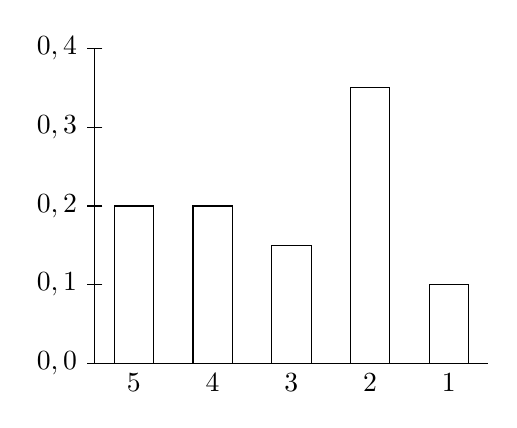
\begin{tikzpicture}
                    \draw (0,0) -- (0,4);
                    \draw (0,0) -- (5,0);
                    \draw (.25,0) rectangle (.75,2);
                    \draw (1.25,0) rectangle (1.75,2);
                    \draw (2.25,0) rectangle (2.75,1.5);
                    \draw (3.25,0) rectangle (3.75,3.5);
                    \draw (4.25,0) rectangle (4.75,1);
                    \node[anchor=north] at (.5,0) {\(5\)};
                    \node[anchor=north] at (1.5,0) {\(4\)};
                    \node[anchor=north] at (2.5,0) {\(3\)};
                    \node[anchor=north] at (3.5,0) {\(2\)};
                    \node[anchor=north] at (4.5,0) {\(1\)};
                    \draw (.1,0) -- (-.1,0) node[left] {\(0,0\)};
                    \draw (.1,1) -- (-.1,1) node[left] {\(0,1\)};
                    \draw (.1,2) -- (-.1,2) node[left] {\(0,2\)};
                    \draw (.1,3) -- (-.1,3) node[left] {\(0,3\)};
                    \draw (.1,4) -- (-.1,4) node[left] {\(0,4\)};
                \end{tikzpicture}
            \end{center}
            \item Der Modalwert ist \(x_\text{mod}\), d.h. die Merkmalsausprägung ``gut'' ist die (hier eindeutig bestimmte) Ausprägung mit maximaler Häufigkeit.
        \end{enumerate}
        \item Kodiert in \(1, \ldots, 5\) ergeben sich die Bewertungen
        \begin{align*}
            x_1 &= 4, & x_2 &= 1, & x_3 &= 2, & x_4 &= 3, & x_5 &= 2, & x_6 &= 1, & x_7 &= 2, & x_8 &= 5, & x_9 &= 5, & x_{10} &= 4,\\
            x_{11} &= 2, & x_{12} &= 3, & x_{13} &= 2, & x_{14} &= 4, & x_{15} &= 5, & x_{16} &= 4, & x_{17} &= 5, & x_{18} &= 2, & x_{19} &= 3, & x_{20} &= 2.
        \end{align*}
        Die zugehörige Rangwertreihe ist gegeben durch
        \begin{align*}
            x_{\parentheses*{1}} &= 1, & x_{\parentheses*{2}} &= 1, & x_{\parentheses*{3}} &= 2, & x_{\parentheses*{4}} &= 2, & x_{\parentheses*{5}} &= 2, & x_{\parentheses*{6}} &= 2, & x_{\parentheses*{7}} &= 2, & x_{\parentheses*{8}} &= 2,\\ 
            x_{\parentheses*{9}} &= 2, & x_{\parentheses*{10}} &= 3, & x_{\parentheses*{11}} &= 3, & x_{\parentheses*{12}} &= 3, & x_{\parentheses*{13}} &= 4, & x_{\parentheses*{14}} &= 4, & x_{\parentheses*{15}} &= 4, & x_{\parentheses*{16}} &= 4,\\
            &&&& x_{\parentheses*{17}} &= 5, & x_{\parentheses*{18}} &= 5, & x_{\parentheses*{19}} &= 5, & x_{\parentheses*{20}} &= 5.
        \end{align*}
        Sind allgemein \(u_1, \ldots, u_m\) die verschiedenen Ausprägungen, dann ist für \(j \in \braces*{1, \ldots, m}\) der Rang \(R\parentheses*{u_j}\) von der Ausprägung \(u_j\) das arithmetische Mittel der Positionen der Werte \(u_j\) in der Rangwertreihe.
        Hier ist \(m = 5\) und speziell \(u_j = j\) für \(j \in \braces*{1, \ldots, 5}\).
        Damit ergibt sich gemäß Vorlesung:
        \begin{center}
            \begin{tabular}{lccccc}
                \toprule
                Merkmalsausprägung \(j\) & \(1\) & \(2\) & \(3\) & \(4\) & \(5\)\\
                \midrule
                Rang \(R\parentheses*{j}\) & \(1,5\) & \(6\) & \(11\) & \(14,5\) & \(18,5\)\\
                \bottomrule
            \end{tabular}
        \end{center}
        Tabelle der Ränge zu allen zwanzig Kodierten Bewertungen:
        \begin{center}
            \begin{tabular}{lccccccccccc}
                \toprule
                Beobachtungsnummer \(j\) & \(1\) & \(2\) & \(3\) & \(4\) & \(5\) & \(6\) & \(7\) & \(8\) & \(9\) & \(10\)\\
                Beobachtungswert \(x_j\) & \(4\) & \(1\) & \(2\) & \(3\) & \(2\) & \(1\) & \(2\) & \(5\) & \(5\) & \(4\)\\
                \midrule
                Rang \(R\parentheses*{x_j}\) & \(14,5\) & \(1,5\) & \(6\) & \(11\) & \(6\) & \(1,5\) & \(6\) & \(18,5\) & \(18,5\) & \(14,5\)\\
                \bottomrule
            \end{tabular}
        \end{center}
        \begin{center}
            \begin{tabular}{lccccccccccc}
                \toprule
                Beobachtungsnummer \(j\) & \(11\) & \(12\) & \(13\) & \(14\) & \(15\) & \(16\) & \(17\) & \(18\) & \(19\) & \(20\)\\
                Beobachtungswert \(x_j\) & \(2\) & \(3\) & \(2\) & \(4\) & \(5\) & \(4\) & \(5\) & \(2\) & \(3\) & \(2\)\\
                \midrule
                Rang \(R\parentheses*{x_j}\) & \(6\) & \(11\) & \(6\) & \(14,5\) & \(18,5\) & \(14,5\) & \(18,5\) & \(6\) & \(11\) & \(6\)\\
                \bottomrule
            \end{tabular}
        \end{center}
    \end{enumerate}


    \section*{Aufgabe 4}

    \begin{problem}
        In einer Befragung von Studierenden wurde ermittelt, mit welchem der folgenden Verkehrsmittel sie die längste Teilstrecke ihres Weges zur Universität zurücklegen:
        \[
            P = \text{PKW}, \quad B = \text{Bus}, \quad Z = \text{Zug}, \quad U = \text{U-Bahn}, \quad R = \text{Fahrrad}, F = \text{``Zu Fuß''}.
        \]
        Hierbei sollte sich jeder der Studierenden fur eines der Verkehrsmittel entscheiden, und aus den insgesamt 200 Angaben resultierten die in der folgenden Tabelle dargestellten prozentualen Anteile:
        \begin{center}
            \begin{tabular}{cccccc}
                \toprule
                \(P\) & \(B\) & \(Z\) & \(U\) & \(R\) & \(F\)\\
                \midrule
                \(12,5\%\) & \(17,5\%\) & \(12,5\%\) & \(10\%\) & \(25\%\) & \(22,5\%\)\\
                \bottomrule
            \end{tabular}
        \end{center}
        \begin{enumerate}
            \item Berechnen Sie die zugehörigen absoluten Häufigkeiten für die einzelnen Verkehrsmittel.
            \item Bei einer Nachkontrolle wurde festgestellt, dass zwei der Studierenden sowohl \(B\) als auch \(R\) angegeben hatten.
            Berechnen Sie die prozentualen Anteile für die Verkehrsmittel-Nutzung, die sich ergeben, wenn die beiden Studierenden mit den doppelten Angaben aus der Umfrage ausgeschlossen werden.
        \end{enumerate}
    \end{problem}

    \subsection*{Lösung}
    \begin{enumerate}
        \item Es bezeichnen \(n_1, \ldots, n_6\) die absoluten und \(f_1, \ldots, f_6\) die relativen Häufigkeiten der sechs Merkmalsausprägungen \(P, B, Z, U, R, F\) (in dieser Reihenfolge).
        Dann gilt gemäß der Vorlesung mit \(n = 200\):
        \[
            f_i = \frac{n_i}{n} \iff n_i = nf_i, \quad i \in \braces*{1, \ldots, 6}.
        \]
        Hiermit erhält man:
        \begin{center}
            \begin{tabular}{lcccccc}
                \toprule
                Verkehrsmittel & \(P\) & \(B\) & \(Z\) & \(U\) & \(R\) & \(F\)\\
                \midrule
                absolute Häufigkeit & \(n_1 = 25\) & \(n_2 = 35\) & \(n_3 = 25\) & \(n_4 = 20\) & \(n_5 = 50\) & \(n_6 = 45\)\\
                \bottomrule
            \end{tabular}
        \end{center}
        \item Da die beiden Studierenden jeweils sowohl \(B\) als auch \(R\) angegeben haben, sind die absoluten Häufigkeiten zu diesen beiden Verkehrsmitteln jeweils um \(2\) zu reduzieren.
        (Nennerumfang wird nun \(\tilde{n} = 196\).)
        Es bezeichnen \(\tilde{n}_1, \ldots, \tilde{n}_6\) bzw. \(\tilde{f}_1, \ldots, \tilde{f}_6\) die neuen absoluten bzw. relativen Häufigkeiten, die sich durch diese Korrektur ergeben.
        Dann ergibt sich mit \(\tilde{n} = 196\):
        \[
            \tilde{f}_i = \frac{\tilde{n}_i}{\tilde{n}}, \quad i \in \braces*{1, \ldots, 6}.
        \]
        Damit erhält man folgende neue Tabelle:
        \begin{center}
            \begin{tabular}{lccccccc}
                \toprule
                Verkehrsmittel & \(P\) & \(B\) & \(Z\) & \(U\) & \(R\) & \(F\)\\
                \midrule
                abs. Häufigkeit & \(\tilde{n}_1 = 25\) & \(\tilde{n}_2 = 33\) & \(\tilde{n}_3 = 25\) & \(\tilde{n}_4 = 20\) & \(\tilde{n}_5 = 48\) & \(\tilde{n}_6 = 45\)\\
                rel. Häufigkeit & \(\tilde{f}_1 = 0,128\) & \(\tilde{f}_2 = 0,168\) & \(\tilde{f}_3 = 0,128\) & \(\tilde{f}_4 = 0,102\) & \(\tilde{f}_5 = 0,245\) & \(\tilde{f}_6 = 0,23\)\\
                Prozentanteile & \(12,8\%\) & \(16,8\%\) & \(12,8\%\) & \(10,2\%\) & \(24,5\%\) & \(23\%\)\\
                \bottomrule
            \end{tabular}
        \end{center}
    \end{enumerate}
\end{document}
